\newcommand{\makeSampleFig}{%
\begin{figure}[tb]
 \centering % avoid the use of \begin{center}...\end{center} and use \centering instead (more compact)
 
\includegraphics[width=\columnwidth]{sample}
 \caption{A visualization of the 1990--2015 data from \autoref{tab:vis_papers}. The image is from \cite{Isenberg:2017:VMC} and is in the public domain.}
 \label{fig:sample}
\end{figure}}

\newcommand{\makeBasicPlottingFig}{%
\begin{figure*}[!btp]
 \centering
% \includegraphics[width=\linewidth]{basicPlotting}
 \includegraphics[width=1.0\textwidth]{figures/basicPlotting.pdf}
 \caption{A selection of basic plots from PyQtGraph's suite of examples.}
 \label{fig:basicPlotting}
\end{figure*}}

\newcommand{\makePtreeExFig}{%
\begin{figure}[!htbp]
\centering
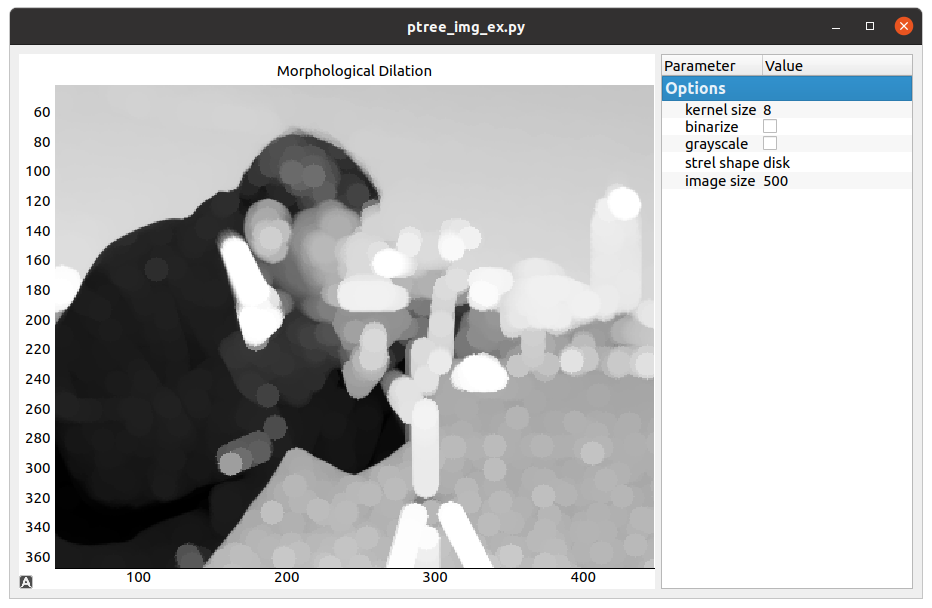
\includegraphics[width=\columnwidth]{figures/pg_ptree_ex}
\caption{Sample use case of parameter trees for function interaction, where various image processing parameters can be quickly updated. Of note, the displayed image reflects these changes in real-time.}
 \label{fig:ptreeEx}
\end{figure}}

\newcommand{\makeLineBenchmarkFig}{
\begin{figure}[!b]
\centering
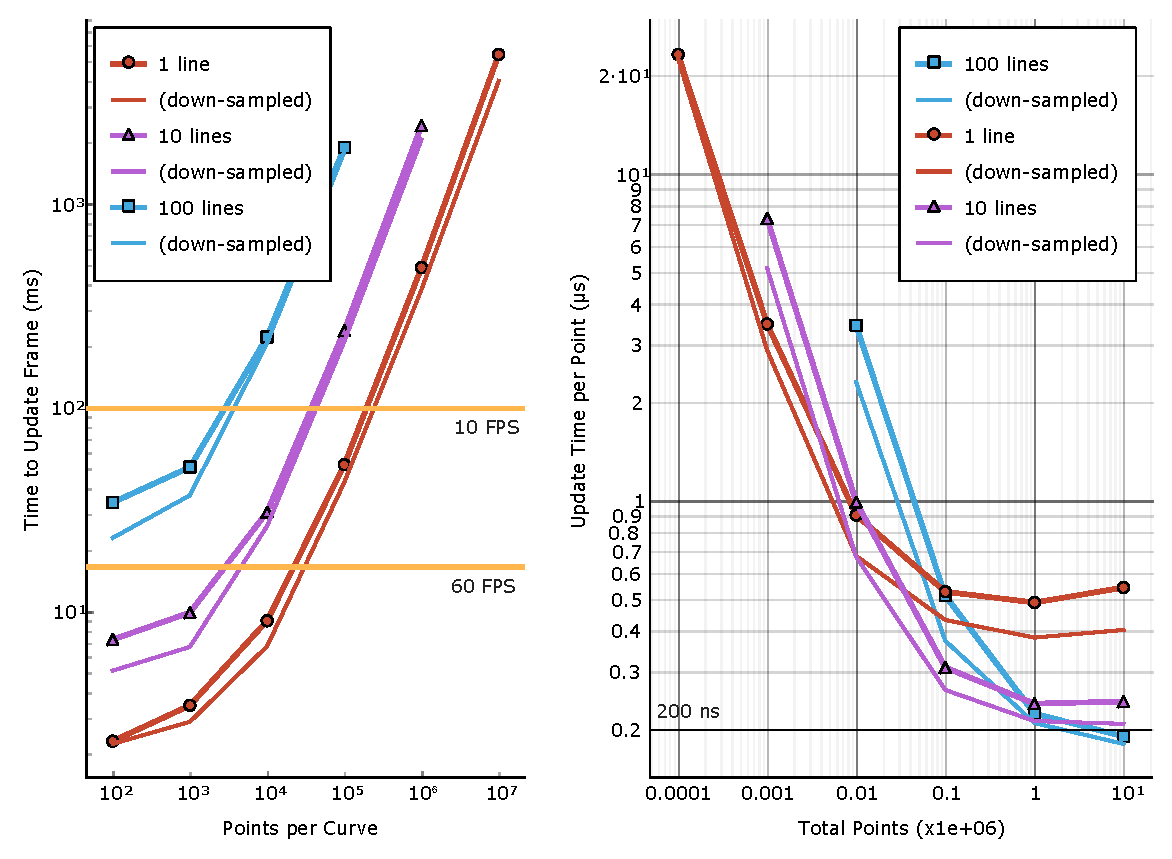
\includegraphics[width=\columnwidth]{figures/lineBenchmark}
\caption{Line speed benchmark. The time to render 1, 10 or 100 lines of data is shown for varying numbers of points per line. All data was collected on a 2020 MacBook Pro with i5 Processor. Left: Time per update over points per curve. The thresholds for achieving 10 and 60 frames/s are shown by horizontal lines. Right: Update time per point, plotted over the total number of points. For more than 100,000 points, the line-plotting time becomes dominant, and the results converge to 200\,ns per point for both 10 and 100 curves, while plotting all points as a single curve increases the time to 500--600 ns\,per point.}
 \label{fig:lineSpeed}
\end{figure}}
 %13-inch 
 
\newcommand{\makeMatplotlibComparison}{%
\begin{figure*}[!bt]
\centering
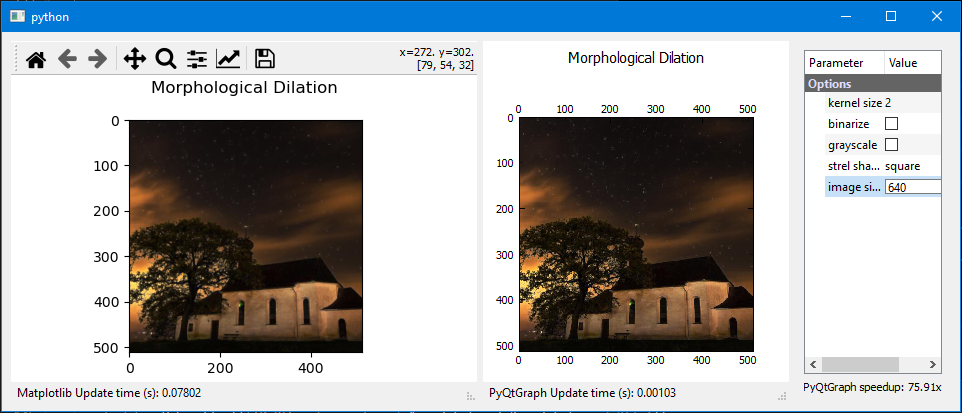
\includegraphics[width=0.8\textwidth]{figures/pg-mpl-comparison}
\caption{Performance test with PyQtGraph and Matplotlib widgets embedded in a Qt5 application. Over a wide range of image sizes, PyQtGraph completes drawing approximately 75--150 times faster, even without hardware acceleration. }
 \label{fig:mpl}
\end{figure*}}

\newcommand{\makeMonitoringFig}{%
\begin{figure}[!htbp]
\centering
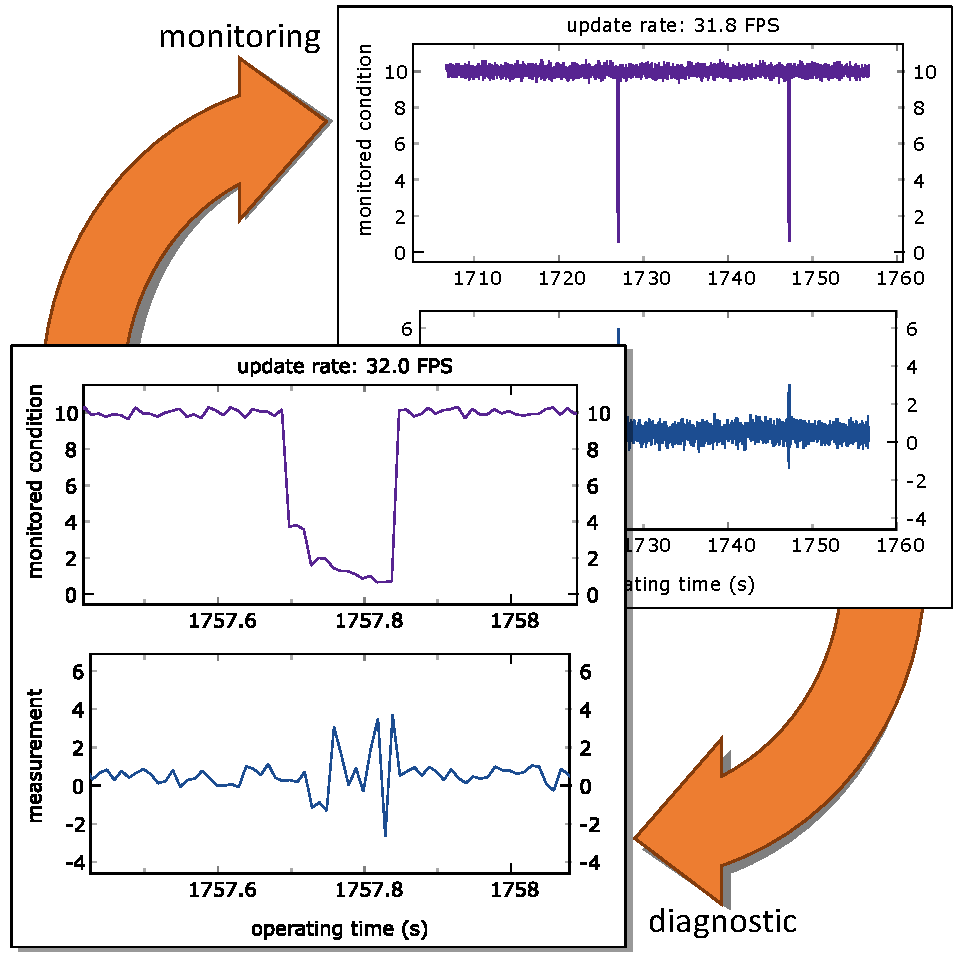
\includegraphics[width=\columnwidth]{figures/monitoring_example_vector.pdf}
\caption{Monitoring and diagnostic of a (simulated) experiment with intermittent failures. Incoming data at 100 samples/s for two measurement channels is recorded into a rolling 5,000 point buffer and continuously displayed at 30 frames/s. When a failure is observed, it can quickly be brought into focus with simple mouse interactions (click-and-drag and mousewheel zoom) for inspection, or to record accurate time stamps. Afterwards, a single click returns the view to automatic scaling without loss of any incoming data.}
 \label{fig:monitoring}
\end{figure}}
